\chapter{Esercizi}
\section{Creare un rete}
\begin{figure}[!htb]
    \centering
    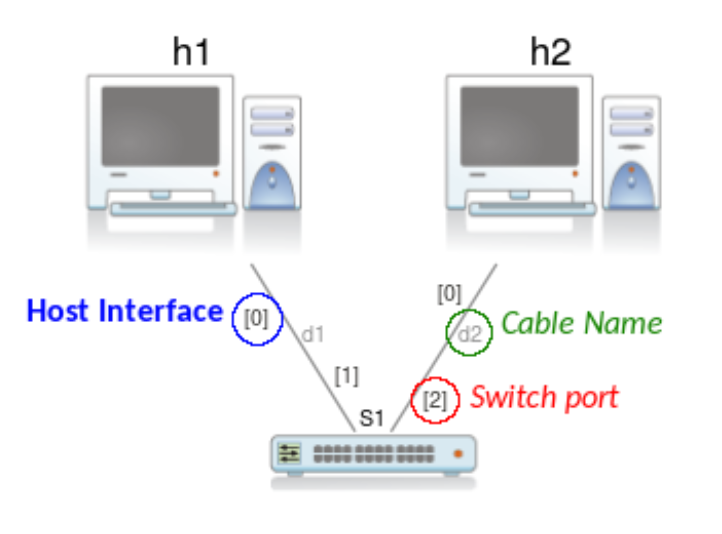
\includegraphics[width=0.4\linewidth]{Images/Esercizi/Marionet.png}
    \caption{Esempio di una rete in Marionet.}
\end{figure}

In Marionet ci sono due tipolgie di cavi:
\begin{enumerate}
    \item \textbf{Cavi crossover:} per connettere macchine sullo stesso livello dello stack.
    \item \textbf{Cavi normali:} per connettere macchine su livelli diversi dello stack.
\end{enumerate}